\documentclass[a4paper,14pt]{extarticle}
\usepackage[utf8]{inputenc}
\usepackage[russian]{babel}
\usepackage{graphicx}
\begin{document}
    Параметры:
    \begin{itemize}
        \item Напряжение на аноде 300В
        \item Напряжение на второй сетке 150В
        \item Диапазон изменения напряжения сетки \( -1\pm0.5\) В
        \item Амплитуда выходного напряжения 100В
    \end{itemize}

    \begin{figure}
    \begin{center}
        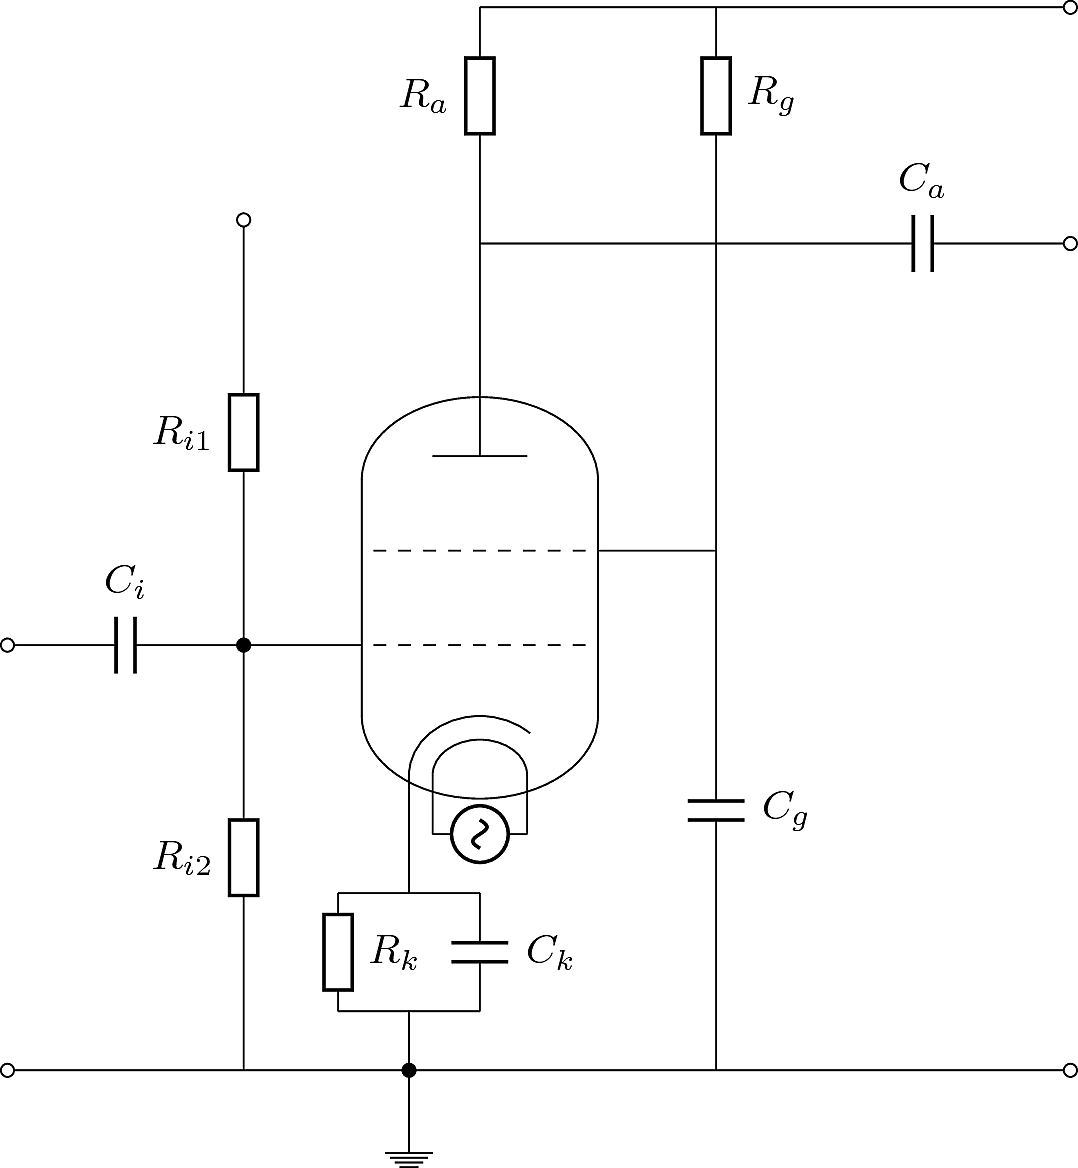
\includegraphics[width=0.7\textwidth]{images/amplifier}
    \end{center}
    \end{figure}

\end{document}
